\documentclass[a4paper,12pt]{article}
\usepackage[T1]{fontenc}
\usepackage[top=3cm, bottom=2cm, left=2cm, right=2cm]{geometry}
\usepackage{fancyhdr}
\usepackage{graphicx}
%\usepackage{appendix} 

\pagestyle{fancyplain}
\usepackage{hyperref}

%%% HEADERS & FOOTERS
\pagestyle{fancy} % options: empty , plain , fancy
\renewcommand{\headrulewidth}{0.5pt} % customise the layout...
\renewcommand{\footrulewidth}{0.5pt} % customise the layout...
\lhead{\emph{Olivier Cl\'{e}ro, Benoit Mass\'{e}, Arthur Templ\'{e}}}\chead{}\rhead{}
\lfoot{\emph{T-111.5350 - MultiMedia Programming}}\cfoot{}\rfoot{\thepage}



%Custom itemize to get less space between items
\newenvironment{my_itemize}{
\begin{itemize}
	\setlength{\topsep}{0pt}
	\setlength{\itemsep}{3pt}
	\setlength{\parskip}{0pt}
	\setlength{\parsep}{0pt}}
{\end{itemize}
}

\newenvironment{my_enumerate}{
\begin{enumerate}
     \setlength{\itemsep}{3pt}
     \setlength{\parskip}{0pt}
     \setlength{\parsep}{0pt}}
{\end{enumerate}
}

\newenvironment{my_description}{
\begin{description}
	\setlength{\topsep}{0pt}
	\setlength{\itemsep}{3pt}
	\setlength{\parskip}{0pt}
	\setlength{\parsep}{0pt}}
{\end{description}
}

%End of custom itemize

\title{  {\large T-111.5350 - MultiMedia Programming}\\~\\
		
\includegraphics[width=0.75\textwidth]{images/logo-with-text.pdf}\\
		A draw-and-guess game for the Aalto Window Station
	}

\begin{document}

\maketitle\thispagestyle{fancy}

%%%%%%%%%%%%%%%%%% INTRODUCTION %%%%%%%%%%%%%%%%%%

\section*{Overview}

The development was achieved by the AaltoWindraw team, formed by Benoit Mass\'{e}, Olivier Cl\'{e}ro and Arthur Templ\'{e} during fall 2012. This project is part of the course T-111.5350 Multimedia Programming at Aalto University. Basically, it is a port of classic boardgame Pictionary to the Aalto Window platform. Rules are the following :
\begin{my_itemize}
\item Two players (or two teams)
\item One of them has to draw something
\item The other has to guess what this something is
\end{my_itemize}
It is similar to another famous mobile game: Draw Something (Android, iPhone).

\section*{Hardware}
This application requires a Windows machine with a touch screen, such as Microsoft Surface, or PixelSense. Aalto Window Platforms are Microsoft PixelSense tables enhanced by some powerful tools (Kinect, MT4J and other multitouch APIs) and located on the three campus of Aalto University, in Espoo (Finland).

\section*{Framework \& Third-party Libraries}
AaltoWindraw was conceived with Microsoft WPF framework. Thus, code is only C\# and XAML, and uses Microsoft Surface SDK 2.0. It is articulated upon a client-server architecture to allow online multiplayer gaming.

Server is dedicated and its database is powered up by MongoDB\footnote{MongoDB's website: \href{http://www.mongodb.org/}{http://www.mongodb.org/}}. Client-server communication is made with Lidgren Network\footnote{Lidgren Network's google code repo: \href{http://code.google.com/p/lidgren-network-gen3/}{http://code.google.com/p/lidgren-network-gen3/}} and JSON.

\section*{How to setup}
In order to run AaltoWindraw, you need an instance of MongoDB running aside AaltoWindraw. Nevertheless, AaltoWindraw itself will raise up an instance of MongoDB if it is not running (provided it is reachable via the PATH variable). An new database is filled \emph{de facto} with a set of default words so that users do not have to manually add them from the beginning.

Some options are to be manually defined according to your needs, they are present in the file: \verb$AaltoWindrawModel/Properties/Resources.resx$. This way the game can be relatively fine-tuned (name of the station, IP of the server, threshold for word recognition and so on).


\section*{Further information}
You can get further information about our project following these links:
\begin{description}
\item[Presentation video on Youtube] \hfill \\ \href{http://www.youtube.com/watch?v=72FyK5rsrqo}{http://www.youtube.com/watch?v=72FyK5rsrqo}
\item[Source code on Github] \hfill \\ \href{https://github.com/TheAaltoWindrawTeam/AaltoWindraw}{https://github.com/TheAaltoWindrawTeam/AaltoWindraw}
\end{description}

\section*{Screenshots}


\begin{minipage}[b]{0.45\linewidth}
\centering
\fbox{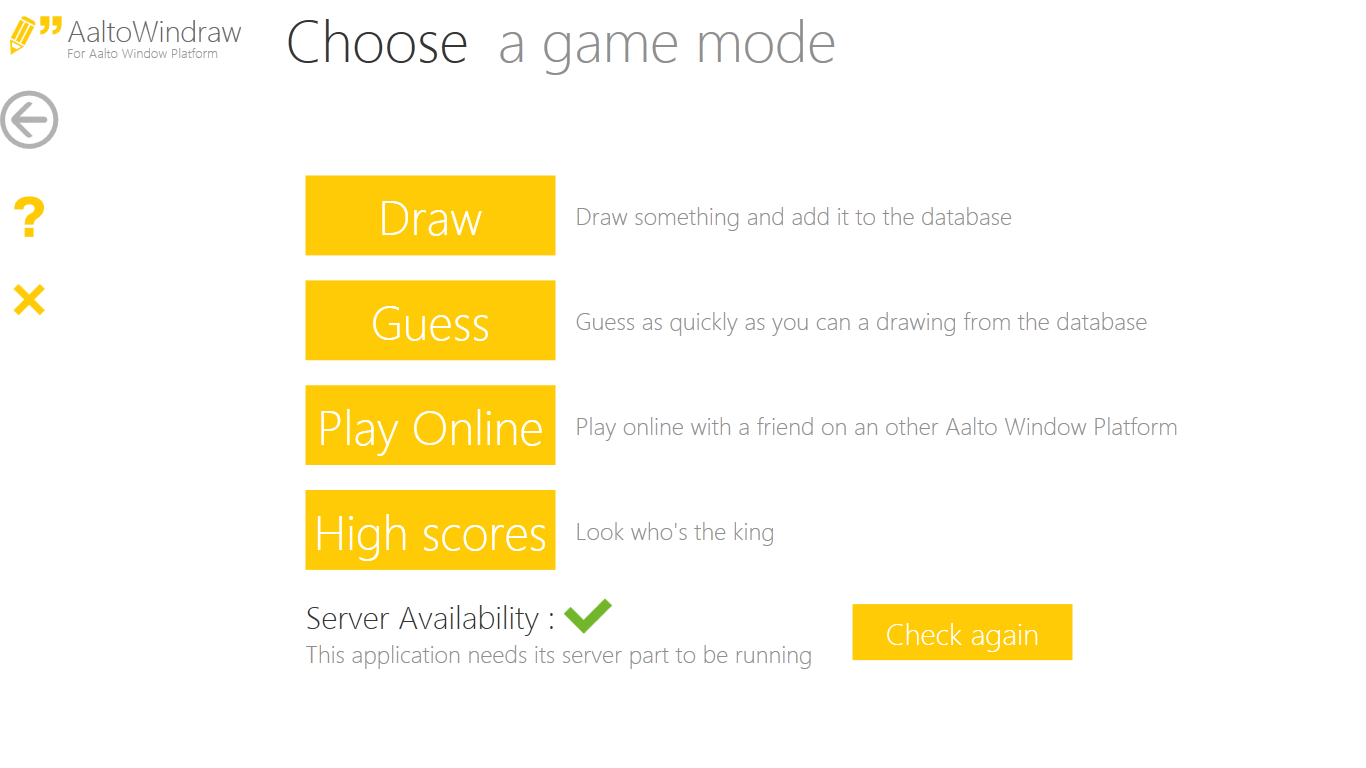
\includegraphics[width=\textwidth]{images/screen1.png}}
\end{minipage}
\hspace{0.5cm}
\begin{minipage}[b]{0.45\linewidth}
\centering
\fbox{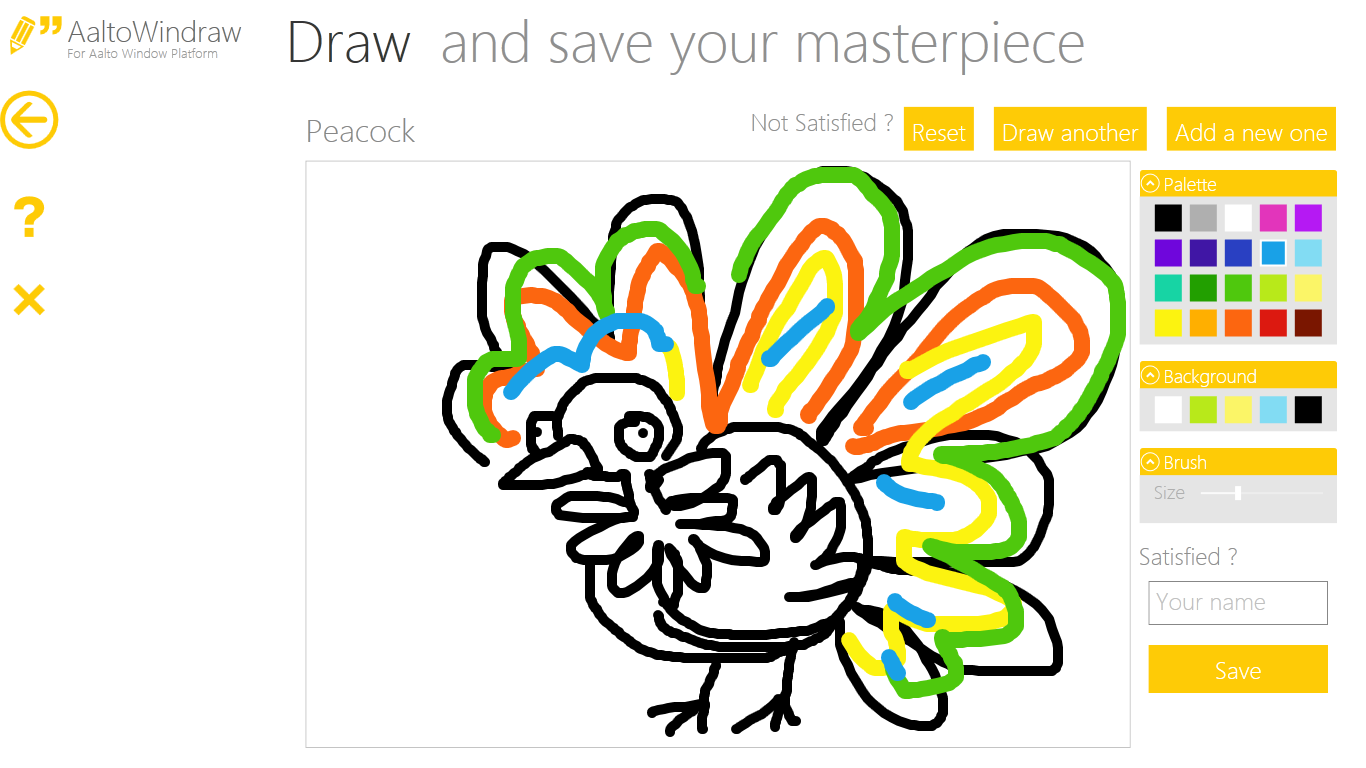
\includegraphics[width=\textwidth]{images/screen2.png}}
\end{minipage}
~\\~\\
\begin{minipage}[b]{0.45\linewidth}
\centering
\fbox{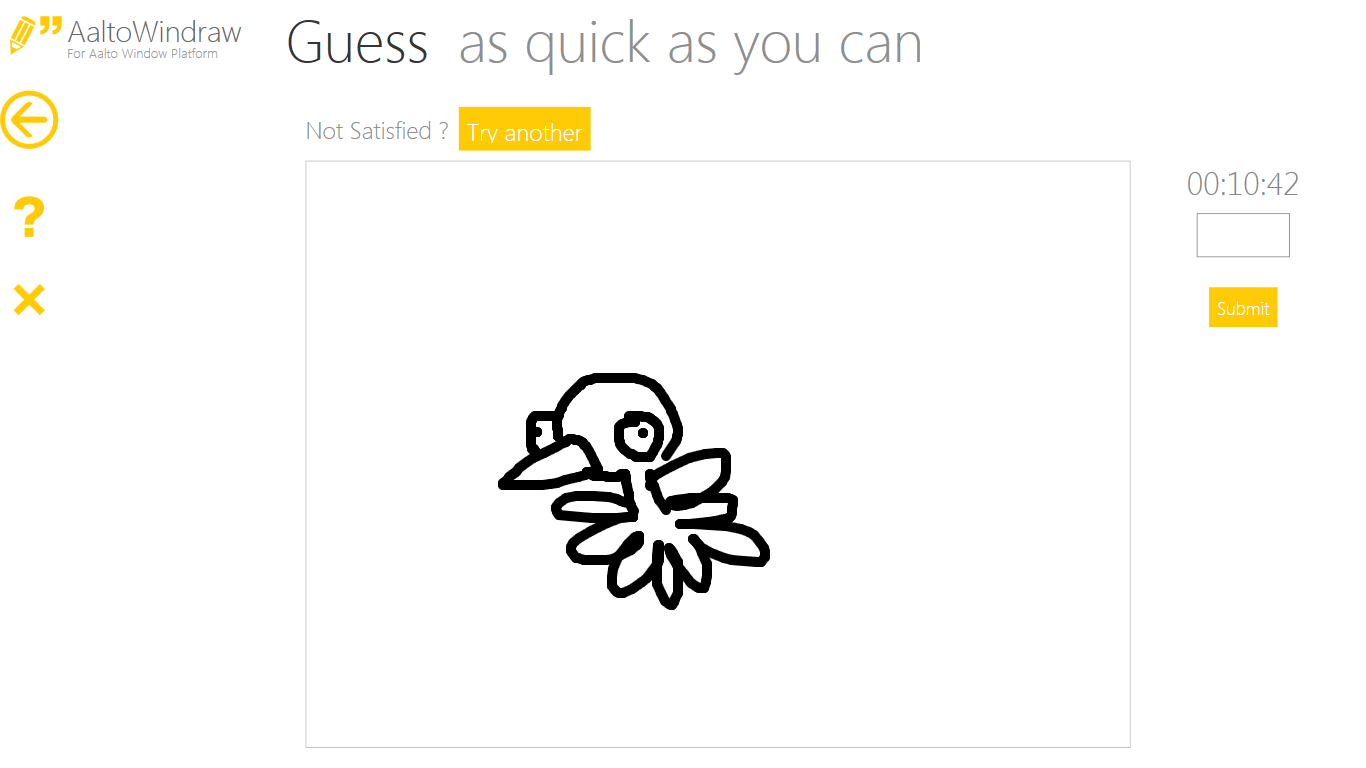
\includegraphics[width=\textwidth]{images/screen3.png}}
\end{minipage}
\hspace{0.5cm}
\begin{minipage}[b]{0.45\linewidth}
\centering
\fbox{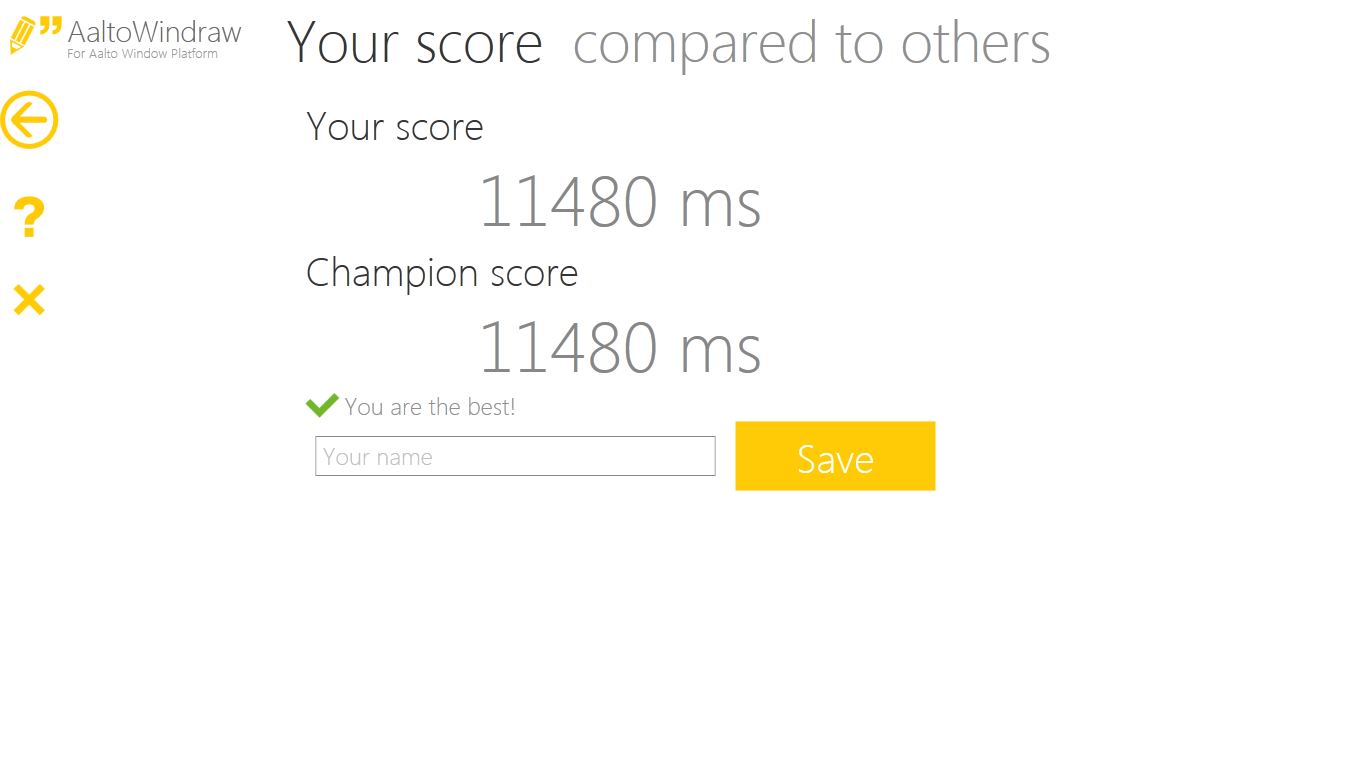
\includegraphics[width=\textwidth]{images/screen4.png}}
\end{minipage}

\end{document}
